% THIS IS SIGPROC-SP.TEX - VERSION 3.1
% WORKS WITH V3.2SP OF ACM_PROC_ARTICLE-SP.CLS
% APRIL 2009
%
% It is an example file showing how to use the 'acm_proc_article-sp.cls' V3.2SP
% LaTeX2e document class file for Conference Proceedings submissions.
% ----------------------------------------------------------------------------------------------------------------
% This .tex file (and associated .cls V3.2SP) *DOES NOT* produce:
%       1) The Permission Statement
%       2) The Conference (location) Info information
%       3) The Copyright Line with ACM data
%       4) Page numbering
% ---------------------------------------------------------------------------------------------------------------
% It is an example which *does* use the .bib file (from which the .bbl file
% is produced).
% REMEMBER HOWEVER: After having produced the .bbl file,
% and prior to final submission,
% you need to 'insert'  your .bbl file into your source .tex file so as to provide
% ONE 'self-contained' source file.
%
% Questions regarding SIGS should be sent to
% Adrienne Griscti ---> griscti@acm.org
%
% Questions/suggestions regarding the guidelines, .tex and .cls files, etc. to
% Gerald Murray ---> murray@hq.acm.org
%
% For tracking purposes - this is V3.1SP - APRIL 2009

\documentclass{proseminar}
\usepackage[hidelinks]{hyperref}
\usepackage[utf8]{inputenc}
\usepackage[T1]{fontenc}
\usepackage{graphicx}

\DeclareGraphicsExtensions{.pdf}

\begin{document}

\conferenceinfo{Albert-Ludwigs Universit\"at Freiburg\\Technische Fakult\"at, Institut f\"ur Informatik\\Lehrstuhl f\"ur Datenbanken \& Informationssysteme}{}

\title{Expos\'e}
\subtitle{outlining a Master Thesis on:\\Semantic approaches to scientific citation recommendation (tentative title)}

\numberofauthors{1}
\author{Tarek Saier\\Reviewer: Prof. Dr. Georg Lausen\\Advisor: Dr.-Ing. Michael Färber}

\maketitle

\section{Introduction}
This expos\'e will outline a prospective master thesis in the area of scientific citation recommendation and argue for its value. The approach will encompass the creation of a dataset and development of supervised learning methods with a focus on semantic analysis of citation contexts. Evaluation of the resulting implementation will follow the most prevalent methods in the field.

The remainder of this document is structured as follows. Section 2 will provide some theoretical background in relevant areas and give a quick overview of related work. A detailed description of the planned methodology and approach will be given in section 3; followed in section 4 by an outline of the planned evaluation. Section 5 and 6 conclude the expos\'e by listing the expected contributions of the thesis and a proposed schedule.

\section{Background}
With the ever increasing number of papers being published it is becoming harder and harder to attain and keep an overview of relevant works within a particular field. As a consequence the difficulty of ensuring the use of appropriate citations and necessary time to do so is getting higher. This is the problem that citation recommendation tries to address.

\subsection{Citation recommendation}
The goal of citation recommendation is to provide adequate citations to a given input text. This can involve evaluating whether or not a given input text includes parts that are suitable to add citations to in the first place. For a given section of or position in an input text, the ouput recommendation can either be a single citation or a ranked list of multiple possible citations. A further distinction can be made concerning the granularity of text that a citation is recommended for. This can range from a complete document (global citation recommendation) to a specific point within a string of text (context aware/local citation recommendation). There are also approaches where citation markers---annotations in the text that mark the position of a citation---are left in the input text. In such a case the evaluation whether or not a citation should be recommended as well as the decision where exactly to put a citation are not necessary. In an ideal case, citation recommendation can even involve evaluating candididate documents in terms of their quality.

Given there are a lot of dimensions along which approaches can differ, section \ref{terminology} will explain relevant terminology and section \ref{dimensions} will give an overview of these distinguishing dimensions. This will enable a more easily understandable overview of related work and explanation of the relative position of the presented approach.

\subsection{Semantic analysis}
The idea of this thesis is to focus on semantic aspects of citation contexts. This means, rather than taking into account only syntactical aspects like n-grams, the analysis will go to a higher level of abstraction where the input's \emph{meaning} is of importance. Because the focus of this analysis will most likely revolve around entities, claims and arguments, these terms will be defined in the following section.

\subsection{Terminology}\label{terminology}
\paragraph{Citing/cited document}
The former is the document making a reference while the latter the document being referenced. The contents of both can be taken into account when developing a citation recommendation approach.

\paragraph{Citation context}
Within the citing document and concerning a single recommendation being made, this is the extend of text provided as input. Examples would be the citing documents abstract, a sentence containing a citation marker or a whole document.

\paragraph{Citation marker}
A citation marker is an annotation in the input text (or a data set) that marks the location of a citation. In scientific publications this could, for example, be a \emph{[42]}. When left in the input text for a recommendation process, the marker's association to its corresponding reference entry is, of course, removed (e.g. \emph{[42]} could be changed to \emph{[]}, replaced by another type of annotation or the citing document's reference section could be made unavailable during the processing of the input). Such a decoupled citation marker is also referred to as \emph{citation placeholder}.

\paragraph{Reference}
For each citation marker there usually is a corresponding reference at the bottom of the page or near the end of the document. This reference identifies the cited document.

\paragraph{Citation function}
The role of a citation or, put differently, the motivation that was behind putting a citation in a particular place. This can, for example, be just for referencing a data set that was used (by citing a data paper), backing up a claim or arguing for or against the overall proposition of a publication.

\paragraph{Metadata}
In addition to a document's content, information \emph{about} the document is also often taken into consideration during the recommendation process. This is referred to as metadata.

\paragraph{Entity}
A physical or abstract thing in the real world. Generally speaking entities like for example people, places, events and topics can be of interest.

\paragraph{Claim}
In this setting a claim can be defined as an assertion which can be judged in tems of its factuality. While non-factual claims also exist (i.e. an opinion being stated), they do not need backing up by citations and are therefore not of interest for citation recommendation.

\paragraph{Argument}
An argument can, in alignment with \cite{Besnard2008}, be defined as being composed of a claim and one or more premises justifying the claim. To illustrate, this can take the form <premises> <step(s) of deduction> <claim> where the claim is the conclusion of the deduction.

\subsection{Dimensions}\label{dimensions}
To systematically categorize approaches to citation recommendation, distinctions can be made concerning the input and the ouput of a mechanism. With regards to the input, the dimensions \emph{citation context} (length/position), \emph{citation markers} (available or not) and \emph{metadata} (available to what extend) can be used. In part, these can be further broken down as shown in the following table.

\begin{table}[!htbp]
\centering
\begin{tabular}{r|c|c}
&learning&use\\ \hline
citing doc & <val> & <val>\\ \hline
cited doc & <val> & <val>\\
\end{tabular}
\end{table}

That is, citing and cited documents can be looked at separately, and a distinction can be made as to what is available during the learning phase and what needs to be provided as input during actual use of the resulting system. Note that for citation markers and context, only the \emph{citing doc} row is applicable\footnote{The term ''citation context'' is used to refer to the context in the citing document. One could make a point, though, to furthermore introduce the notion of a context in the cited document. This could then be used, for example, to distinguish whether or not a mechanism outputs only a recommended document or also a specific section that is relevant; or to distinguish whether or not (parts of) cited documents are used during the learning phase.} and for metadata most likely only the \emph{learning} column is\footnote{Although metadata aspects like the ''date of the citing doc'' could also be used in the online system. That is, given a newly written text without citations, an approach could interpret the input as a ''recent citing doc'' and recommend citations accordingly.}. Because dimensions along tree axis are hard to visualize effectively, the distinction can be flattened to the following aspects:

\begin{itemize}
    \item citation context (learning)
    \item citation context (use)
    \item citation markers (learning)
    \item citation markers (use)
    \item metadata (citing doc)
    \item metadata (cited doc)
\end{itemize}

To give a concrete example, an approach could be trained on input with citation markers (citation markers (learning)),  but be able to give useful output for input without markers (citation markers (use)) as well.

Above example also suggests, that there is a distinction to be made concerning an approaches output. A dimension \emph{citation placement granularity} can be used to distinguish whether citation recommendations are given for a whole document, on a sentence level or if specific points within the text are identified.

\subsection{Related work}\label{relwork}
\cite{Faerber} (F\"arber et al.) offers a comprehensive overview of the field of citation recommendation as well as a comparison of concrete approaches. Focus in the following will be works with distinct similarities or differences to the proposed approach (explained in section \ref{meth}) which are therefore helpful in defining it.

Mishra et al. describe in \cite{Mishra2016} an approach to recommend news articles that can be used as references in Wikipedia articles describing historical events. Their goal is to offer readers an insight into the detailed view on and reporting of an event \emph{at the time} as an addition to the more overarching representation on Wikipedia. This approach employs named entities as a key component to identify appropriate news articles to recommend. It is therefore similar in this regard to the first step in the master thesis' approach where the focus also will lie on recommendation based on entities. The domain, being Wikipedia and news articles, differs from scientific publications.

In \cite{Levy2014}, Levy et al. describe a method for claim detection using a cascade of classifiers. The detection of claims will also be necessary in the proposed thesis' second step (citation recommendation based on claims). Levy et al. do, however, restrict their detection of claims to those related to a predefined topic and include claims that are statements of an opinion, which will most likely not be the case in the master thesis.

In a similar fashion Goudas et al. tackle argument extraction in \cite{Goudas2014}, which will need to be done in the thesis' thrid step (citation recommendation based on arguments). The document type being social media texts is, however, different.

Tbahriti et al. semantically analyse abstracts of scientific publications in \cite{Tbahriti2006} to aid the retrieval of similar documents. They classify sentences into one of \emph{purpose}, \emph{methods}, \emph{results} and \emph{conclusion} and show that treating these classes of sentences in a distinct manner can help finding documents with similar references. While mentioning that a system like theirs could also be used for recommending citations, this was not part of the approach. Furthermore, the semantic classes of sentences are identified within the abstract and therefore differ in terms of the citation context from the proposed thesis.

In \cite{Duma2016} Duma et al. apply the rhetorical annotation scheme CoreSC\cite{Liakata2010} (including classes like \emph{hypothesis}, \emph{background}, \emph{me\-thod}, etc.) to citation contexts and use this classification as part of the query when determining the citations to recommend. This determination of the function of a citation within the argumentative structure of an input text is an aspect that is likely going to be part of the master thesis' thrid step (citation recommendation based on arguments). The used citation context length of 3 sentences is likely to be in the realm of what will be used in the master thesis as well. A difference lies in the research domain of the publications used. While Duma et al. use publications from biomedical science, the thesis will most likely use publications form the eight fields found on arxiv.org.

Kobayashi et al. classify citations into three discourse facets (\emph{objective}, \emph{method}, \emph{result}) in \cite{Kobayashi2018}. For their citation recommendation approach they then use facet based vector representations of their citation graph. While, as with \cite{Duma2016}, the rhetorical analysis of citation contexts is a similarity to the proposed thesis, the focus on the citation graph will most likely not be one.

\section{Methodology and approach}\label{meth}
Proposed is a context based citation recommendation approach for scientific publications. In the following subsections considerations concerning the data set and the recommendation process will be explained.

\subsection{Dataset}
In the field of citation recommendation a lot of different datasets are used and there is no real de facto standard as of yet. Following the analysis in \cite{Faerber} it can be seen that each of the more widely used datasets has benefits and drawbacks. Since the proposed approach for the master thesis will involve semantic analysis of citation contexts, the availability of large citation contexts as well as the availability of exact citation markers/placeholders is desirable. \cite{Faerber2018} show that based on arXiv.org publication sources it is possible to generate a very clean and reliable dataset for citation recommendation. Their approach involving linking publications to DBLP restricts them, however, to only use one of the eight domains available on arXiv.org (namely computer science) resulting in only a medium sized data set. The PubMedCentral Open Access collection\footnote{http://www.ncbi.nlm.nih.gov/pmc/tools/openftlist/} also offers publication source files, but in an already processed XML format.

Going for size, another possible approach would be to use a matadata set like the Microsoft Academic Graph\cite{Sinha2015} (MAG), which is very lage \emph{and} contains citations contexts---albeit only with a length of one sentence. An advantage of using the MAG would be, that the citation graph is already built. In case of generating a data set from arXiv.org sources, reference texts would first have to be linked to publications. \cite{Herrmannova2016} report, however, that in case of the MAG, 80 out of the 127 million papers have neither references nor citations.

Considering the above, the use of arXiv.org sources (1.4 M documents) or PubMedCentral Open Access sources (2.1 M documents) as well as the use of the MAG (30 M connected entities of document metadata) could be considered. Advantages of the MAG are the already built citation graph\footnote{Although, given the MAG is generated automatically, relying on this pre-built graph could be seen as making an approach less transparent.} and its size. The citation context length of just one sentence is a bit small. It might be possible to work on an intersection of MAG and publication sources and thereby extend the citation contexts (utilizing the MAG's pre-built graph structure and the sources' full text), but this would then negate the size argument. Advantages of a dataset generated from source files are the freedom to decide on arbitrarily large citation contexts, the availability of citation markers and the transparency of the approach. Here, the pre-processed nature of the PubMedCentral Open Access collection takes away part of the transparency. A general drawback is the necessity to match references (which in the end are just arbitrary strings input by authors) with publications to generate a citation graph.

Considering the size of citation contexts used in other approaches that semantically analyse them like \cite{Duma2016} and \cite{Kobayashi2018}, it could be argued that generating a dataset based on arXiv.org sources is the most promising approach for the goal at hand. While the PubMedCentral Open Access collection looks like a viable alternative to arXiv.org sources, the lack of familiarity with the dataset would necessitate additional checks and analysis to make a resonably justified decision between the two. The proposed generation of a dataset will therefore look as follows.

\subsubsection{Generating a dataset from arXiv.org sources}
arXiv.org sources are availabe for bulk download and consist, for the most part, of LaTeX source files. There are, however, publications for which there's only TeX, DVI, PostScript or HTML sources or even just a PDF. Where LaTeX source files are available they can be either converted into XML by software like LaTeXML\footnote{https://github.com/brucemiller/LaTeXML} or Tralics\footnote{https://www-sop.inria.fr/marelle/tralics/} to generate plain text with citation annotations from XML, or parsed by libraries like plastex\footnote{https://github.com/tiarno/plastex} or TexSoup\footnote{https://github.com/alvinwan/texsoup}, skipping the inbetween XML format. In case of a restriction to computer science publications, grabcite\footnote{https://github.com/agrafix/grabcite} could be used as a tool for the whole dataset generation process.

For the general case, after parsing the LaTeX sources and obtaining plain text with citation annotations, the reference strings corresponding to these citations still need to be resolved (i.e. matched to some set of global IDs). For citations \emph{within} the publications on arXiv.org (i.e. matching to arXiv IDs), this can for example be done by indexing the publications' metadata with a software like Apache Lucene\footnote{https://lucene.apache.org/} and then querying the resulting indices with the reference strings. Because some LaTeX sources include arXiv IDs in their bibliographies this step is not necessary every time.

In a preliminary test with 10270 citations from 377 publications posted to arXiv in December 2017, 315 of the reference entries already included arXiv IDs and a further 1703 could be matched with the technique described above. While this is only close to 20\%, optimistically extrapolating the numbers to the complete 1.4 M documents in arXiv this would still result in a dataset of 7.6 M citations.

\subsubsection{Extension with the MAG}
In addition to publication sources, arXiv.org also offers structured metadata on their publications. The MAG, being a metadata set, could be used to enrich this metadata. This could be beneficial for the recommendation process, would however require a matching of arXiv IDs to MAG IDs. Gauging prospective gains and feasibility will be a task further down the line.

\subsection{Recommendation}
\subsubsection{Categorization}
Categorizing the proposed approach according to the dimensions defined in section \ref{dimensions}, it would look as follows:

\begin{itemize}
    \item citation context (learning): in accordance with what will turn out to be effective when using entities, claims, arguments or any combination of those. Gauging by related approaches this is probably going to be in the realm of one two a few sentences.
    \item citation context (use): how much input the system will need in order to produce useful output, can hardly be estimated at this point.
    \item citation markers (learning): will be provided at their exact position, because the dataset will be generated from LaTeX sources.
    \item citation markers (use): whether citation placeholders will be needed in the input or whether the approach will include a mechanism to decide on where to put citations is still open.
    \item metadata (citing doc): will be available\footnote{https://arxiv.org/help/oa/arXiv\_meta\_format.html}
    \item metadata (cited doc): same as above
\end{itemize}

\subsubsection{Overview}
The gist of how the proposed recommendation process will look like is illustrated in figure \ref{fig:schema}. The dataset is built from LaTeX source files and is comprised of plain text with special annotations for citations. This means per citation we can obtain a citation context (i.e. surrounding text) of appropriate length. The idea is then to learn an abstract representation of those citation contexts. A query to the resulting system is then similarly mapped onto its abstract representation and compared to all the citation contexts in the data set. With this comparison the most similar contexts can be identified and their respective citations recommended.

\begin{figure}[h!]
 \centering
 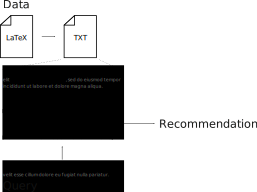
\includegraphics[scale=0.3]{img/recommendation_process_schema}
 \caption{Schematic view on the recommendation process of citations.}
 \label{fig:schema}
\end{figure}

Abovementioned abstract representations of citation contexts will be created in such a way that they capture the text's semantic content. To be more precise, first an approach will be developed to identify entities. Second, the same will be done for claims and lastly arguments will be captured. The basic idea is that for the same citations are usable for similar semantic surroundings (e.g. the same claim backed up by the same citation).

As mentioned in capter \ref{relwork}, \cite{Mishra2016} by Mishra et al. is an example for the use of entities as an indicator to find relevant citations, an example of claim detection can be seen in \cite{Levy2014} by Levy et al. and in \cite{Goudas2014} Goudas et al. tackle argument extraction.

\subsubsection{Machine learning approach}
The machine learning approach will need to allow for the integration of comparatively explicitly modeled concepts (entities, claims, arguments). Furthermore the separate development of approaches (again, for entities, claims, arguments) and their combination afterwards has to be possible. One option would therefore be to go with engineering features that capture abovementioned semantic concepts and use these in a vector space model.

\section{Evaluation}
A straightforward approach to evaluating the resulting recommender system is re-prediction of citations. As is the norm with evaluating machine learning approaches the data is split into a training and testing set. While the training set is left ''intact'' the citations are removed from the test set (citation placeholders might be left in place). The system then trains on the training set and tries to re-predict the citations in the test set that were originally there (or rather, recommend a list of fitting citations). To get more reliable results, above procedure is not just performed with one random split but in the manner of a k-fold cross-validation.

To measure the quality of the resulting recommendation a combination of a ''hard'' measure like \emph{top-1 accuracy} and a more ''soft'' measure like \emph{normalized discounted cumulative gain} (NDCG)\footnote{Making good use of NDCG might necessitate defining a relevance measure for recommendations that differ from the original one.} can be used.

If possible, it would be ideal to also test the resulting appraoch on existing datasets to allow for a direct comparison of performance. Whether this is a possibility or not will have to be assessed when the project has made some progress and there are less unknowns.

\section{Contributions}
As can be seen in \cite{Faerber}, the body of work on semantic approaches to scientific citation recommendation is not that large. A contribution of the proposed thesis would therefore be an extension of this body of work.

Furthermore, similar to \cite{Faerber2018}, another contribution will be a high quality dataset that can be used to evaluate citation recommendation approaches. This dataset will also encompass several difference domains of research.

\section{Schedule}
The proposed schedule can be seen in table \ref{schedule}.

\begin{table*}
\centering
\caption{Schedule}\label{schedule}
\hphantom{ }
\begin{tabular}{|p{2.5cm}|p{6cm}|p{4cm}|} \hline
Time frame&Task&Results\\ \hline
Oct 1 -- Oct 21 & Develop mechanism to generate dataset with citation markers from arXiv source dump & Dataset boilerplate (i.e. with citation markers but no semantic annotation)\\ \hline
Oct 22 -- Oct 28 & Write expos\'e  & Thesis approval\\ \hline
Oct 29 -- Nov 04 & Add entity annotations to dataset & Dataset usable for supervised learning\\ \hline
Nov 05 -- Nov 18 & Develop entity based recommendation approach & Basic code boilerplate done and first recommendation process implemented\\ \hline
Nov 19 -- Nov 25 & Add claim annotations to dataset & Added value for the data set\\ \hline
Nov 26 -- Dec 09 & Develop claim based recommendation approach & Second recommendation approach\\ \hline
Dec 10 -- Dec 22 & Coordination with simultaneous tangential theses and integration into CiteRec system & Compatibility of code base\\ \hline
Dec 23 -- Jan 06 & break/buffer & -\\ \hline
Jan 07 -- Jan 13 & Add argument annotations to dataset & Added value for the data set\\ \hline
Jan 14 -- Jan 27 & Develop argument based recommendation approach and start offline evaluation & Thrid recommendation approach\\ \hline
Jan 28 -- Feb 10 & Offline evaluation & Evaluation results\\ \hline
Feb 11 -- Feb 24 & Online evaluation & Evaluation results\\ \hline
Feb 25 -- Mar 17 & Thesis writing & Written thesis\\ \hline
Mar 18 -- Mar 31 & buffer/paper writing & -\\ \hline\end{tabular}
\end{table*}

% \section{}
% \subsection{}
% \subsubsection{}
% \footnote{}
% \begin{math}\lim_{n\rightarrow \infty}x=0\end{math}
% \begin{equation}\lim_{n\rightarrow \infty}x=0\end{equation}
% \begin{displaymath}\sum_{i=0}^{\infty} x + 1\end{displaymath}
% \begin{table}
% \centering
% \caption{Frequency of Special Characters}
% \begin{tabular}{|c|c|l|} \hline
% Non-English or Math&Frequency&Comments\\ \hline
% \O & 1 in 1,000& For Swedish names\\ \hline
% $\pi$ & 1 in 5& Common in math\\ \hline
% \$ & 4 in 5 & Used in business\\ \hline
% $\Psi^2_1$ & 1 in 40,000& Unexplained usage\\
% \hline\end{tabular}
% \end{table}
%
% \begin{table*}
% \centering
% \caption{Some Typical Commands}
% \begin{tabular}{|c|c|l|} \hline
% Command&A Number&Comments\\ \hline
% \texttt{{\char'134}alignauthor} & 100& Author alignment\\ \hline
% \texttt{{\char'134}numberofauthors}& 200& Author enumeration\\ \hline
% \texttt{{\char'134}table}& 300 & For tables\\ \hline
% \texttt{{\char'134}table*}& 400& For wider tables\\ \hline\end{tabular}
% \end{table*}
%
% \begin{figure}
% \centering
% \epsfig{file=fly.eps}
% \caption{A sample black and white graphic (.eps format).}
% \end{figure}
%
% \newtheorem{theorem}{Theorem}
% \begin{theorem}
% Let $f$ be continuous on $[a,b]$.  If $G$ is
% an antiderivative for $f$ on $[a,b]$, then
% \begin{displaymath}\int^b_af(t)dt = G(b) - G(a).\end{displaymath}
% \end{theorem}
%
% \begin{figure*}
% \centering
% \epsfig{file=flies.eps}
% \caption{A sample black and white graphic (.eps format)
% that needs to span two columns of text.}
% \end{figure*}

\bibliographystyle{abbrv}
\bibliography{../paper}  % bibliography.bib is the name of the Bibliography in this case

% remember to run:
% latex bibtex latex latex
% to resolve all references
%
% ACM needs 'a single self-contained file'!

\balancecolumns
\end{document}
